\documentclass[12pt,]{article}
\usepackage{lmodern}
\usepackage{amssymb,amsmath}
\usepackage{ifxetex,ifluatex}
\usepackage{fixltx2e} % provides \textsubscript
\ifnum 0\ifxetex 1\fi\ifluatex 1\fi=0 % if pdftex
  \usepackage[T1]{fontenc}
  \usepackage[utf8]{inputenc}
\else % if luatex or xelatex
  \ifxetex
    \usepackage{mathspec}
  \else
    \usepackage{fontspec}
  \fi
  \defaultfontfeatures{Ligatures=TeX,Scale=MatchLowercase}
    \setmainfont[]{Times New Roman}
\fi
% use upquote if available, for straight quotes in verbatim environments
\IfFileExists{upquote.sty}{\usepackage{upquote}}{}
% use microtype if available
\IfFileExists{microtype.sty}{%
\usepackage{microtype}
\UseMicrotypeSet[protrusion]{basicmath} % disable protrusion for tt fonts
}{}
\usepackage[margin=2.54cm]{geometry}
\usepackage{hyperref}
\hypersetup{unicode=true,
            pdftitle={UV Absorbance characteristics in Northern Lakes},
            pdfauthor={Rachel Bash},
            pdfborder={0 0 0},
            breaklinks=true}
\urlstyle{same}  % don't use monospace font for urls
\usepackage{color}
\usepackage{fancyvrb}
\newcommand{\VerbBar}{|}
\newcommand{\VERB}{\Verb[commandchars=\\\{\}]}
\DefineVerbatimEnvironment{Highlighting}{Verbatim}{commandchars=\\\{\}}
% Add ',fontsize=\small' for more characters per line
\usepackage{framed}
\definecolor{shadecolor}{RGB}{248,248,248}
\newenvironment{Shaded}{\begin{snugshade}}{\end{snugshade}}
\newcommand{\KeywordTok}[1]{\textcolor[rgb]{0.13,0.29,0.53}{\textbf{#1}}}
\newcommand{\DataTypeTok}[1]{\textcolor[rgb]{0.13,0.29,0.53}{#1}}
\newcommand{\DecValTok}[1]{\textcolor[rgb]{0.00,0.00,0.81}{#1}}
\newcommand{\BaseNTok}[1]{\textcolor[rgb]{0.00,0.00,0.81}{#1}}
\newcommand{\FloatTok}[1]{\textcolor[rgb]{0.00,0.00,0.81}{#1}}
\newcommand{\ConstantTok}[1]{\textcolor[rgb]{0.00,0.00,0.00}{#1}}
\newcommand{\CharTok}[1]{\textcolor[rgb]{0.31,0.60,0.02}{#1}}
\newcommand{\SpecialCharTok}[1]{\textcolor[rgb]{0.00,0.00,0.00}{#1}}
\newcommand{\StringTok}[1]{\textcolor[rgb]{0.31,0.60,0.02}{#1}}
\newcommand{\VerbatimStringTok}[1]{\textcolor[rgb]{0.31,0.60,0.02}{#1}}
\newcommand{\SpecialStringTok}[1]{\textcolor[rgb]{0.31,0.60,0.02}{#1}}
\newcommand{\ImportTok}[1]{#1}
\newcommand{\CommentTok}[1]{\textcolor[rgb]{0.56,0.35,0.01}{\textit{#1}}}
\newcommand{\DocumentationTok}[1]{\textcolor[rgb]{0.56,0.35,0.01}{\textbf{\textit{#1}}}}
\newcommand{\AnnotationTok}[1]{\textcolor[rgb]{0.56,0.35,0.01}{\textbf{\textit{#1}}}}
\newcommand{\CommentVarTok}[1]{\textcolor[rgb]{0.56,0.35,0.01}{\textbf{\textit{#1}}}}
\newcommand{\OtherTok}[1]{\textcolor[rgb]{0.56,0.35,0.01}{#1}}
\newcommand{\FunctionTok}[1]{\textcolor[rgb]{0.00,0.00,0.00}{#1}}
\newcommand{\VariableTok}[1]{\textcolor[rgb]{0.00,0.00,0.00}{#1}}
\newcommand{\ControlFlowTok}[1]{\textcolor[rgb]{0.13,0.29,0.53}{\textbf{#1}}}
\newcommand{\OperatorTok}[1]{\textcolor[rgb]{0.81,0.36,0.00}{\textbf{#1}}}
\newcommand{\BuiltInTok}[1]{#1}
\newcommand{\ExtensionTok}[1]{#1}
\newcommand{\PreprocessorTok}[1]{\textcolor[rgb]{0.56,0.35,0.01}{\textit{#1}}}
\newcommand{\AttributeTok}[1]{\textcolor[rgb]{0.77,0.63,0.00}{#1}}
\newcommand{\RegionMarkerTok}[1]{#1}
\newcommand{\InformationTok}[1]{\textcolor[rgb]{0.56,0.35,0.01}{\textbf{\textit{#1}}}}
\newcommand{\WarningTok}[1]{\textcolor[rgb]{0.56,0.35,0.01}{\textbf{\textit{#1}}}}
\newcommand{\AlertTok}[1]{\textcolor[rgb]{0.94,0.16,0.16}{#1}}
\newcommand{\ErrorTok}[1]{\textcolor[rgb]{0.64,0.00,0.00}{\textbf{#1}}}
\newcommand{\NormalTok}[1]{#1}
\usepackage{longtable,booktabs}
\usepackage{graphicx,grffile}
\makeatletter
\def\maxwidth{\ifdim\Gin@nat@width>\linewidth\linewidth\else\Gin@nat@width\fi}
\def\maxheight{\ifdim\Gin@nat@height>\textheight\textheight\else\Gin@nat@height\fi}
\makeatother
% Scale images if necessary, so that they will not overflow the page
% margins by default, and it is still possible to overwrite the defaults
% using explicit options in \includegraphics[width, height, ...]{}
\setkeys{Gin}{width=\maxwidth,height=\maxheight,keepaspectratio}
\IfFileExists{parskip.sty}{%
\usepackage{parskip}
}{% else
\setlength{\parindent}{0pt}
\setlength{\parskip}{6pt plus 2pt minus 1pt}
}
\setlength{\emergencystretch}{3em}  % prevent overfull lines
\providecommand{\tightlist}{%
  \setlength{\itemsep}{0pt}\setlength{\parskip}{0pt}}
\setcounter{secnumdepth}{5}
% Redefines (sub)paragraphs to behave more like sections
\ifx\paragraph\undefined\else
\let\oldparagraph\paragraph
\renewcommand{\paragraph}[1]{\oldparagraph{#1}\mbox{}}
\fi
\ifx\subparagraph\undefined\else
\let\oldsubparagraph\subparagraph
\renewcommand{\subparagraph}[1]{\oldsubparagraph{#1}\mbox{}}
\fi

%%% Use protect on footnotes to avoid problems with footnotes in titles
\let\rmarkdownfootnote\footnote%
\def\footnote{\protect\rmarkdownfootnote}

%%% Change title format to be more compact
\usepackage{titling}

% Create subtitle command for use in maketitle
\providecommand{\subtitle}[1]{
  \posttitle{
    \begin{center}\large#1\end{center}
    }
}

\setlength{\droptitle}{-2em}

  \title{UV Absorbance characteristics in Northern Lakes}
    \pretitle{\vspace{\droptitle}\centering\huge}
  \posttitle{\par}
  \subtitle{\url{https://github.com/rachelbash/absorbance-data-project}}
  \author{Rachel Bash}
    \preauthor{\centering\large\emph}
  \postauthor{\par}
    \date{}
    \predate{}\postdate{}
  

\begin{document}
\maketitle
\begin{abstract}
Experimental overview. This section should be no longer than 250 words.
What contributes to absorbance values in the NTL\_LTER Carbon data set
(will consider things such as DIC, DOC, depth, and water pressure).
Also, is there a significant change in absorbance values in lakes over
time?
\end{abstract}

\newpage

\tableofcontents  \newpage
\listoftables
1 Data Summary
\ldots{}\ldots{}\ldots{}\ldots{}\ldots{}\ldots{}\ldots{}\ldots{}\ldots{}\ldots{}\ldots{}\ldots{}\ldots{}\ldots{}\ldots{}\ldots{}\ldots{}\ldots{}\ldots{}\ldots{}\ldots{}\ldots{}.6
\newpage
\listoffigures  \newpage

\section{Research Question and
Rationale}\label{research-question-and-rationale}

Absorbance is a unitless measurement that describes how much a substance
absorbs light over a certain range of wavelenght. The absorbance values
of water samples from lakes can provide details regarding its physical
characteristics and the health of the lake. The amount of light entering
a lake is an component that drives photosynthesis and lake metabolism.
Additionally, lake temperature and its absorbance characteristics are
deeply intertwined. With the right equipment, absorbance is fairly easy
to measure. Therefore, measuring absorbance in lakes can give
researchers insight into other processes happening that depend on
sunlight.

This research project intends to answer two main questions: What
contributes to absorbance values in five lakes located in Michigan's
Upper Penninsula? Do absorbance values in these five study lakes change
over time? The data that answer these questions come from the North
Temperate Lakes Project, which seeks to measure data on carbon and other
related variables in lakes. My analysis of the data provides a model
that shows the variables that best predict absorbance values and also
takes a closer look at how absorbance values have changed over time in
different lakes. Time variations in absorbance have implications that
other physical characteristics are changing, which may damage biota in
the lakes or bring about significant changes in the greater ecosystem
that surrounds the lake.

\newpage

\section{Dataset Information}\label{dataset-information}

The dataset was collected from 1984 to 2016 by researchers working for
the Cascade Project and Northern Temperate Lakes at a total of 14 sites.
Samples of water were collected, and then were measured. Measurements
included dissolved organic and inorganic carbon, particulate organic
matter, partial pressure of carbon dioxide, and absorbance. Absorbance
was measured using a spectrophotometer at a wavelength of 440nm.

For some variables, a water depth sample was taken that was measured in
meters, while in others, samples were taken to reflect a depth that was
proportional across all lakes. Therefore, Hypolimnion, Epilimnion,
Metalimnion, and pooled mixed layer (PML) are also included as depth
values. All water samples were taken with a syringe and then filtered
through a mesh filter in order to remove any large debris or
zooplankton.

\begin{longtable}[]{@{}ll@{}}
\toprule
\begin{minipage}[b]{0.26\columnwidth}\raggedright\strut
Data Summary\strut
\end{minipage} & \begin{minipage}[b]{0.30\columnwidth}\raggedright\strut
Relevant Information\strut
\end{minipage}\tabularnewline
\midrule
\endhead
\begin{minipage}[t]{0.26\columnwidth}\raggedright\strut
Date range\strut
\end{minipage} & \begin{minipage}[t]{0.30\columnwidth}\raggedright\strut
1984-06-03 to 2016-08-17\strut
\end{minipage}\tabularnewline
\begin{minipage}[t]{0.26\columnwidth}\raggedright\strut
Structure\strut
\end{minipage} & \begin{minipage}[t]{0.30\columnwidth}\raggedright\strut
15 variables with 13,557 observations\strut
\end{minipage}\tabularnewline
\begin{minipage}[t]{0.26\columnwidth}\raggedright\strut
Column names\strut
\end{minipage} & \begin{minipage}[t]{0.30\columnwidth}\raggedright\strut
lakeid, lakename, year4, daynum, sampledate, depth, depth\_id, tpc, tpn,
DIC\_mg, DIC\_uM, air\_pco2, water\_pco2, doc, absorbance\strut
\end{minipage}\tabularnewline
\begin{minipage}[t]{0.26\columnwidth}\raggedright\strut
Lakes sampled\strut
\end{minipage} & \begin{minipage}[t]{0.30\columnwidth}\raggedright\strut
Crampton Lake, East Long Lake, Hummingbird Lake, Long Lake, Morris Lake,
North Gate Bog, Paul Lake, Peter Lake, Reddington Lake, Roach Lake,
Tender Bog, Tuesday Lake, Ward Lake, West Long Lake\strut
\end{minipage}\tabularnewline
\bottomrule
\end{longtable}

\newpage

\section{Exploratory Data Analysis and
Wrangling}\label{exploratory-data-analysis-and-wrangling}

\paragraph{Importing raw data and identifying its
attributes}\label{importing-raw-data-and-identifying-its-attributes}

\begin{Shaded}
\begin{Highlighting}[]
\CommentTok{#exploratory code to see the full dataset and its attributes}
\KeywordTok{colnames}\NormalTok{(carbon.data)}
\end{Highlighting}
\end{Shaded}

\begin{verbatim}
##  [1] "lakeid"     "lakename"   "year4"      "daynum"     "sampledate"
##  [6] "depth"      "depth_id"   "tpc"        "tpn"        "DIC_mg"    
## [11] "DIC_uM"     "air_pco2"   "water_pco2" "doc"        "absorbance"
\end{verbatim}

\begin{Shaded}
\begin{Highlighting}[]
\KeywordTok{str}\NormalTok{(carbon.data)}
\end{Highlighting}
\end{Shaded}

\begin{verbatim}
## 'data.frame':    13557 obs. of  15 variables:
##  $ lakeid    : Factor w/ 14 levels "E","H","L","Long",..: 3 3 3 3 3 8 8 8 8 8 ...
##  $ lakename  : Factor w/ 14 levels "Crampton Lake",..: 7 7 7 7 7 8 8 8 8 8 ...
##  $ year4     : int  1984 1984 1984 1984 1984 1984 1984 1984 1984 1984 ...
##  $ daynum    : int  155 155 155 155 155 156 156 156 156 156 ...
##  $ sampledate: Date, format: "1984-06-03" "1984-06-03" ...
##  $ depth     : Factor w/ 231 levels "0","0.1","0.15",..: 1 62 102 140 180 1 62 102 140 202 ...
##  $ depth_id  : int  1 2 3 4 5 1 2 3 4 5 ...
##  $ tpc       : num  NA NA NA NA NA NA NA NA NA NA ...
##  $ tpn       : num  NA NA NA NA NA NA NA NA NA NA ...
##  $ DIC_mg    : num  1.45 1.82 1.51 1.47 2.69 2.85 2.84 3.27 2.98 7.26 ...
##  $ DIC_uM    : num  121 152 126 122 224 ...
##  $ air_pco2  : num  NA NA NA NA NA NA NA NA NA NA ...
##  $ water_pco2: num  NA NA NA NA NA NA NA NA NA NA ...
##  $ doc       : num  NA NA NA NA NA NA NA NA NA NA ...
##  $ absorbance: num  NA NA NA NA NA NA NA NA NA NA ...
\end{verbatim}

\begin{Shaded}
\begin{Highlighting}[]
\KeywordTok{summary}\NormalTok{(carbon.data)}
\end{Highlighting}
\end{Shaded}

\begin{verbatim}
##      lakeid               lakename        year4          daynum     
##  R      :3887   Peter Lake    :3887   Min.   :1984   Min.   : 82.0  
##  L      :3852   Paul Lake     :3852   1st Qu.:1993   1st Qu.:166.0  
##  T      :1818   Tuesday Lake  :1818   Median :1999   Median :192.0  
##  W      :1571   West Long Lake:1571   Mean   :2000   Mean   :192.4  
##  E      :1435   East Long Lake:1435   3rd Qu.:2007   3rd Qu.:218.0  
##  M      : 456   Crampton Lake : 456   Max.   :2016   Max.   :310.0  
##  (Other): 538   (Other)       : 538                                 
##    sampledate                 depth         depth_id           tpc        
##  Min.   :1984-06-03   0          :1719   Min.   :-2.000   Min.   : 0.100  
##  1st Qu.:1993-06-16   Metalimnion:1297   1st Qu.: 1.000   1st Qu.: 0.580  
##  Median :1999-07-06   Hypolimnion:1020   Median : 3.000   Median : 0.890  
##  Mean   :2000-07-14   PML        : 876   Mean   : 2.775   Mean   : 1.110  
##  3rd Qu.:2007-08-28   Epilimnion : 570   3rd Qu.: 5.000   3rd Qu.: 1.305  
##  Max.   :2016-08-17   (Other)    :7918   Max.   : 7.000   Max.   :11.860  
##                       NA's       : 157   NA's   :170      NA's   :11410   
##       tpn            DIC_mg           DIC_uM            air_pco2    
##  Min.   :0.000   Min.   : 0.023   Min.   :   1.917   Min.   :197.7  
##  1st Qu.:0.070   1st Qu.: 0.812   1st Qu.:  67.625   1st Qu.:343.4  
##  Median :0.103   Median : 1.322   Median : 110.167   Median :362.9  
##  Mean   :0.149   Mean   : 2.310   Mean   : 192.487   Mean   :360.4  
##  3rd Qu.:0.180   3rd Qu.: 1.968   3rd Qu.: 164.000   3rd Qu.:379.0  
##  Max.   :2.170   Max.   :48.599   Max.   :4049.883   Max.   :608.1  
##  NA's   :11409   NA's   :3642     NA's   :3642       NA's   :12411  
##    water_pco2          doc           absorbance   
##  Min.   :   0.0   Min.   : 2.710   Min.   :0.011  
##  1st Qu.: 478.0   1st Qu.: 4.570   1st Qu.:0.060  
##  Median : 838.5   Median : 5.603   Median :0.146  
##  Mean   :1012.3   Mean   : 6.932   Mean   :0.194  
##  3rd Qu.:1175.6   3rd Qu.: 8.370   3rd Qu.:0.265  
##  Max.   :9348.2   Max.   :44.080   Max.   :1.213  
##  NA's   :12411    NA's   :9993     NA's   :10658
\end{verbatim}

\begin{Shaded}
\begin{Highlighting}[]
\KeywordTok{dim}\NormalTok{(carbon.data)}
\end{Highlighting}
\end{Shaded}

\begin{verbatim}
## [1] 13557    15
\end{verbatim}

\begin{Shaded}
\begin{Highlighting}[]
\KeywordTok{summary}\NormalTok{(carbon.data}\OperatorTok{$}\NormalTok{absorbance)}
\end{Highlighting}
\end{Shaded}

\begin{verbatim}
##    Min. 1st Qu.  Median    Mean 3rd Qu.    Max.    NA's 
##   0.011   0.060   0.146   0.194   0.265   1.213   10658
\end{verbatim}

\begin{Shaded}
\begin{Highlighting}[]
\KeywordTok{class}\NormalTok{(carbon.data}\OperatorTok{$}\NormalTok{depth)}
\end{Highlighting}
\end{Shaded}

\begin{verbatim}
## [1] "factor"
\end{verbatim}

\begin{Shaded}
\begin{Highlighting}[]
\KeywordTok{head}\NormalTok{(carbon.data}\OperatorTok{$}\NormalTok{depth, }\DecValTok{10}\NormalTok{)}
\end{Highlighting}
\end{Shaded}

\begin{verbatim}
##  [1] 0   1   2   3.5 5.5 0   1   2   3.5 7  
## 231 Levels: 0 0.1 0.15 0.17 0.18 0.19 0.2 0.21 0.22 0.23 0.25 0.28 ... surface
\end{verbatim}

These exploratory commands above function as helpful tools that help me
see what kind of shape my data are in. It shows me how many NA's I have,
what variables I am working with, the classes of my variables, and basic
summary statistics. An important thing I discovered while doing the
initial exploratory data analysis is that the depth variable has both
numeric and factor-level observations, which is why its class is listed
as \texttt{factor}. In other words, depth was measured in both numeric
terms (1 meter, 13 meters, etc), but also in thermally stratified terms,
such as Hypolimnion, Metalimnion, and Epilimnion. This was an important
discovery that led to further data wrangling and filtering of this
specific variable.

\paragraph{Visualizing the data}\label{visualizing-the-data}

As seen by \autoref{fig:foo}, Absorbance values are not normally
distributed. This is expected, as we are dealing with ecological data.

\begin{figure}
\centering
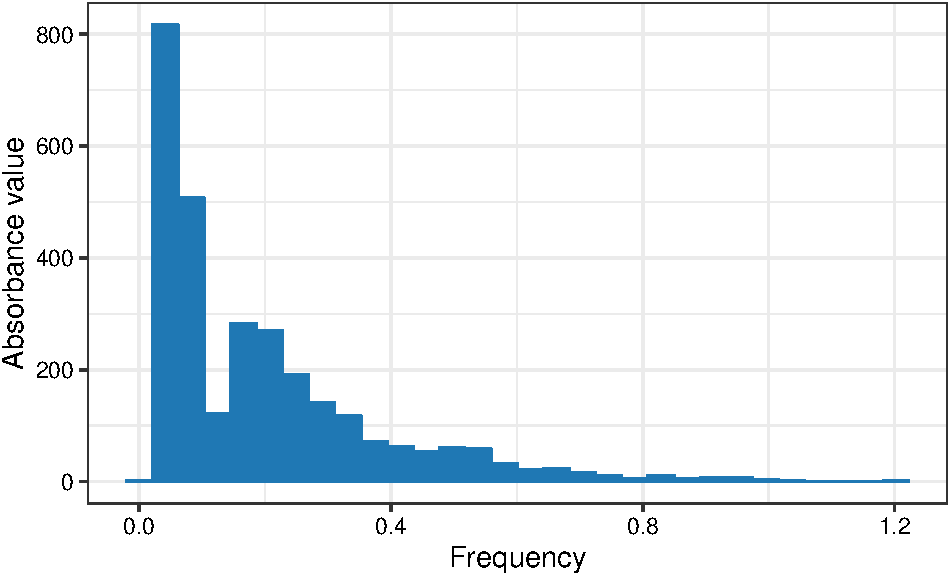
\includegraphics{Bash_ENV872_Project_files/figure-latex/foo-1.pdf}
\caption{\label{fig:foo}Absorbance frequency}
\end{figure}

\begin{figure}
\centering
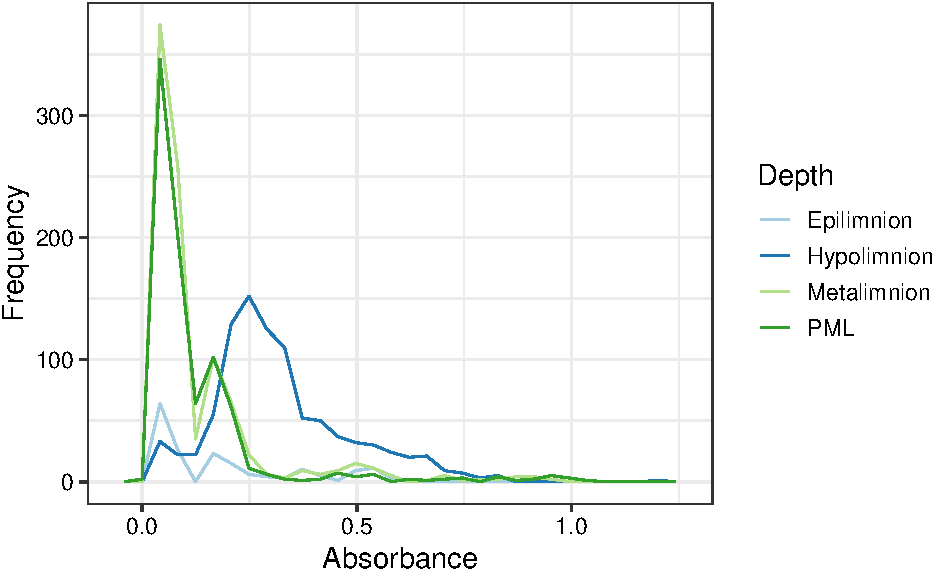
\includegraphics{Bash_ENV872_Project_files/figure-latex/freqpol-1.pdf}
\caption{\label{fig:freqpol}Absorbance frequency by depth category}
\end{figure}

Relatedly, \autoref{fig:freqpol} shows that different levels of depth
(factor) had difference absorbance freqency values. It was helpful to
create this graph to show that absorbance was measured at multiple
different water depth levels.

\begin{figure}
\centering
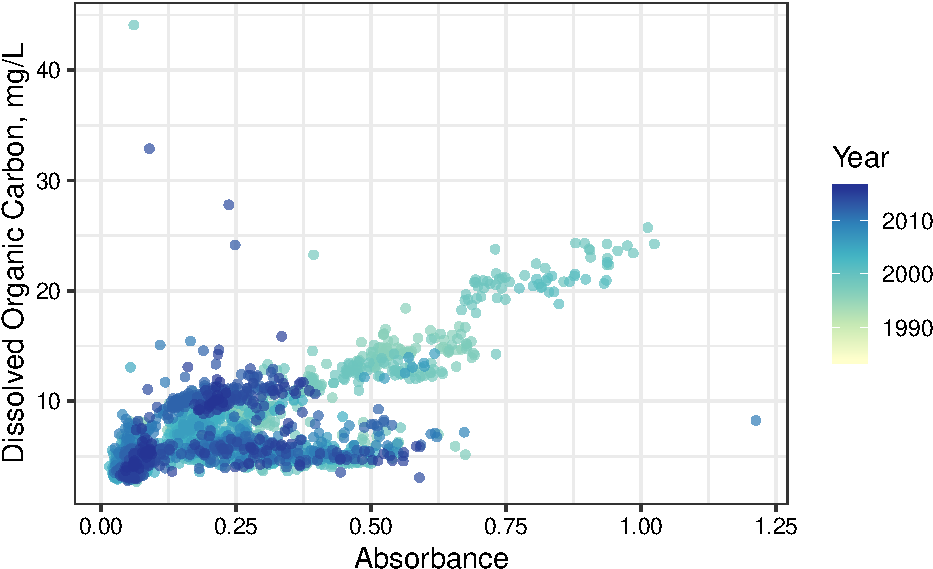
\includegraphics{Bash_ENV872_Project_files/figure-latex/absorbdoc-1.pdf}
\caption{\label{fig:absorbdoc} Disolved organic carbon and absorbance
relationship by year}
\end{figure}

\newpage

\section{Analysis}\label{analysis}

\newpage

\section{Summary and Conclusions}\label{summary-and-conclusions}


\end{document}
